\graphicspath{{figures/design/}}


			\chapter{Test Journal: Servomotors}



\begin{table}[!h]
\begin{tabular}{l l}
\textbf{Test participants:} & Romain \& Raphael   \\
\textbf{Date:}  & 01/05-2017
\end{tabular}
\end{table}




	\section*{Purpose}
The purpose of the test is to verify the proper functionment of the servomotors, and calculate the time constant of the servomotors' required tasks.




	\section*{Test equipment and components}
\begin{table}[h]
	\centering
	\caption{List of measurement equipment and components}\label{tab_appendix:template}

	\begin{tabularx}{\textwidth}{lXXXX}
		Name 				& Brand	& Model 									\\ \toprule \rowcolor{lightGrey}
		Servomotor	& SpringRc & SM-s2309s 	\\
		Controller	& Arduino & Arduino Nano\\ 
		Camera & Samsung & 0\\
		Media Player Classic & Gabest & Home Cinema\\ \rowcolor{lightGrey}
	\end{tabularx}
\end{table}




	\section*{Setup}
Measurement setup is seen on \autoref{fig:DCSetup} and photo \
\begin{figure} [h]
\centering

\includegraphics[width=0.6\linewidth]{figures/frontpage.jpg}
\caption{Measurement setup.}
\label{fig:DCSetup}
\end{figure}

The servos are controlled and powered by an Arduino Uno. Three different position of the servo sticks are set up by code found in the attachements.




	\section*{Method}
 The servos are controlled to go from one position to another set one. The process is filmed in slow motion in order to analyse it. 




	\section*{Raw data}
	
		\subsubsection*{Angle variation}

\begin{figure} [htbp]
	\centering
	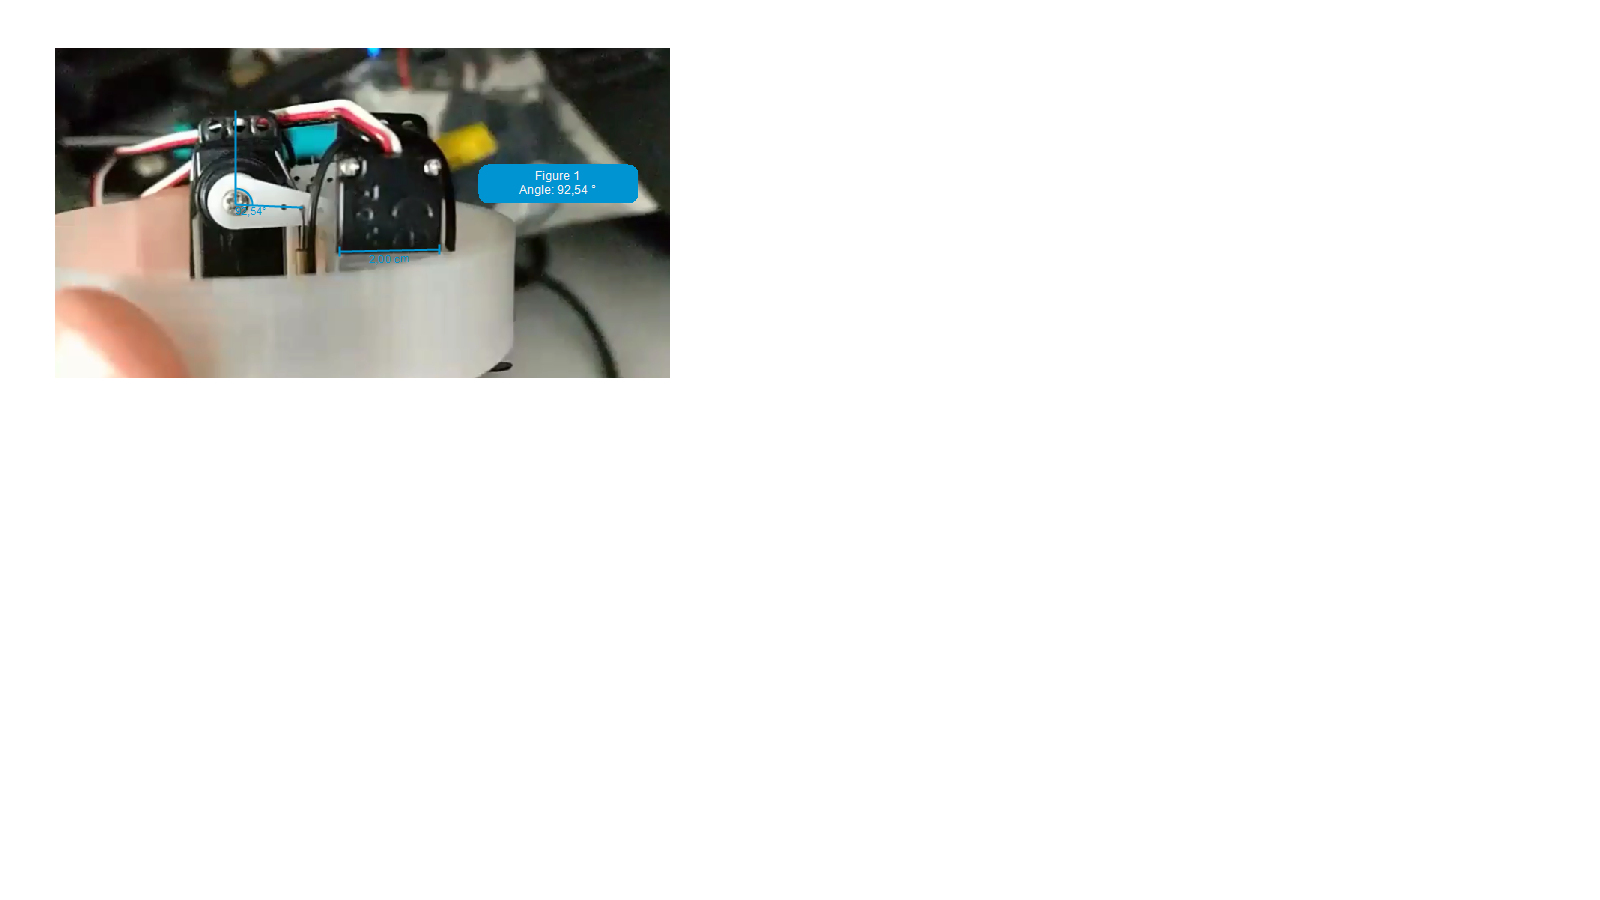
\includegraphics[width=0.35\linewidth]{figures/"Rocket"/"Servomotors"/middlepositionangle.png}
	\caption{Photograph of the servomotor at the medium position.} \label{fig:ServoInitialPosition}
\end{figure}

\begin{figure} [htbp]
	\centering
	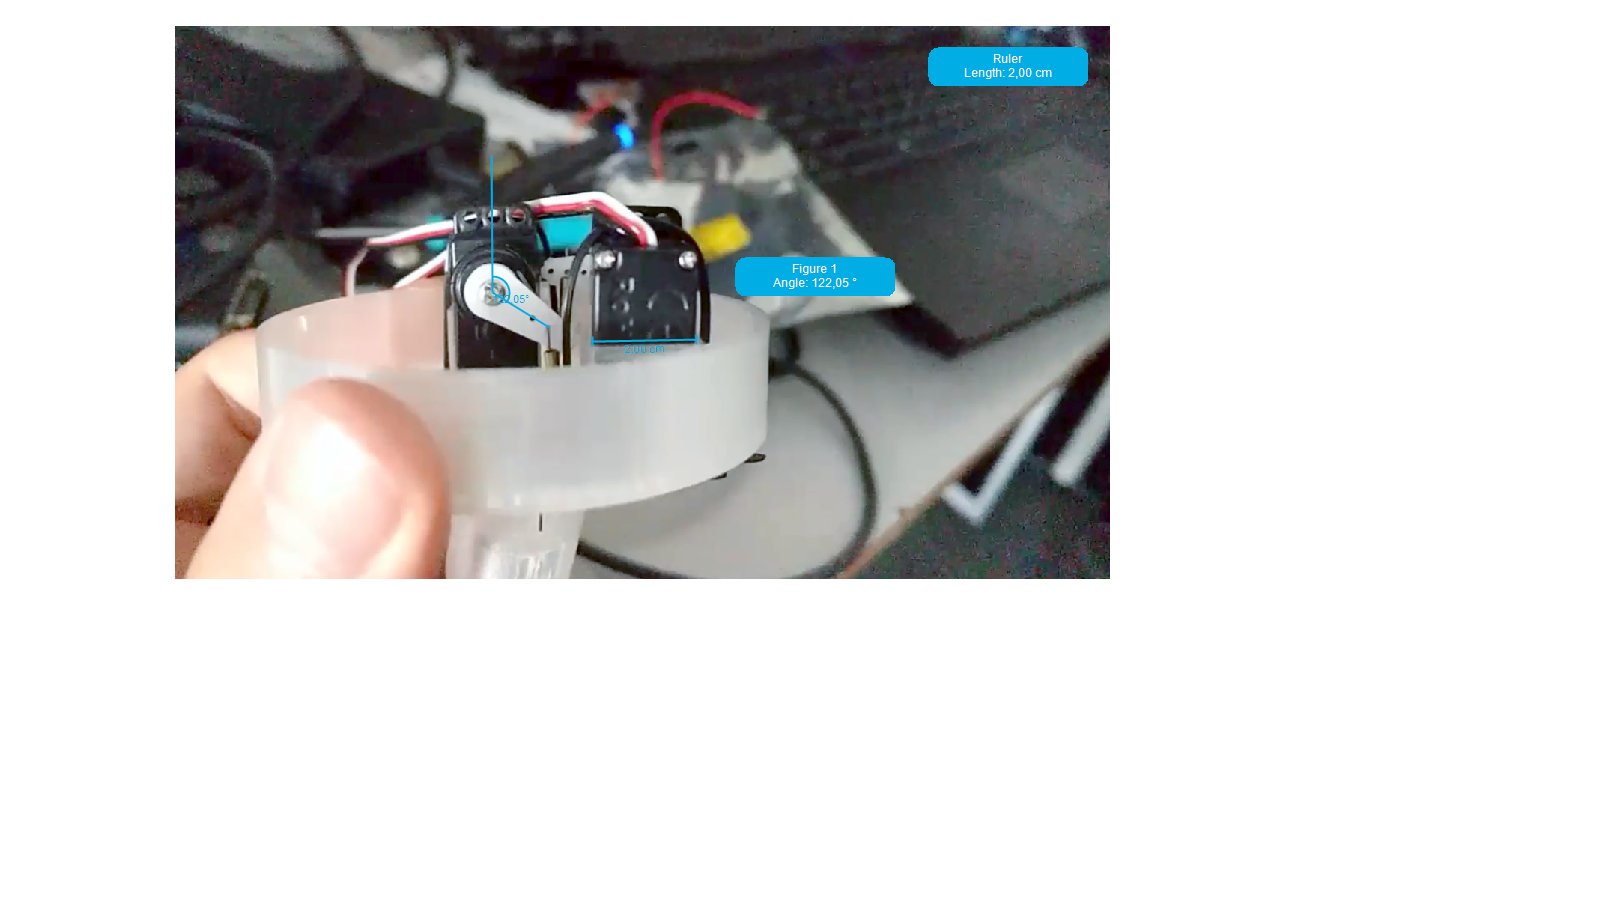
\includegraphics[width=0.35\linewidth]{figures/"Rocket"/"Servomotors"/downpositionangle.png}
	\caption{Photograph of the servomotor at the lower position.} \label{fig:ServoLowPosition}
\end{figure}

\begin{figure} [htbp]
	\centering
	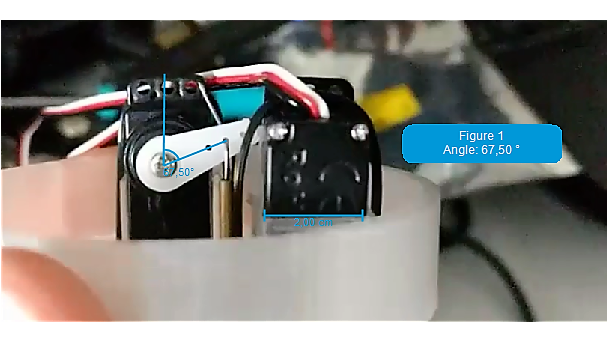
\includegraphics[width=0.35\linewidth]{figures/"Rocket"/"Servomotors"/highpositionangle.png}
	\caption{Photograph of the servomotor at the higher position.} \label{fig:ServoHighPosition}
\end{figure}

		\subsubsection*{Time constant}




	\section*{Data processing}	
\subsubsection*{Angle variation}
The angle variation is also found by measuring the angle difference betwwen the horizontal axis and the stick direction. The servomotors function properlly if the angles desired correspond to the real angles.
\subsubsection*{Time constant}
 In order to find the time constant, the time to go from one position to another is measured using the video software. The time constant is equal to 63 per cent of the total time from one position to another. 
 
 
 

	\section*{Conclusion}
The servomotors follow the requirements, and are considered valid. The total time from one position to another is. The time constant is then .





